% multiple1902 <multiple1902@gmail.com>
% intro.tex
% Copyright 2011~2012, multiple1902 (Weisi Dai)
% https://code.google.com/p/xjtuthesis/
% 
% It is strongly recommended that you read documentations located at
%   http://code.google.com/p/xjtuthesis/wiki/Landing?tm=6
% in advance of your compilation if you have not read them before.
%
% This work may be distributed and/or modified under the
% conditions of the LaTeX Project Public License, either version 1.3
% of this license or (at your option) any later version.
% The latest version of this license is in
%   http://www.latex-project.org/lppl.txt
% and version 1.3 or later is part of all distributions of LaTeX
% version 2005/12/01 or later.
%
% This work has the LPPL maintenance status `maintained'.
% 
% The Current Maintainer of this work is Weisi Dai.
%

\chapter{系统需求分析}
\echapter{Analysis}
\label{AnalysisChapter}
\section{系统需求}
\setcounter{subsubsection}{0}
\subsubsection{局部性(Locality)}
\par
根据游戏设计,每个节点应当具有一个球形的感知范围(Area of interest)。节点应当只收到落在自己的感知范围内的对象的位置和行动的更新。不仅如此,如前\ref{kNNIntroSection}部分所述,由于整个游戏的虚拟空间过大,其中包含的节点过多,希望每一个节点获取整个虚拟空间的全部状态信息是不现实的。此要求即为游戏虚拟环境的局部性要求。该要求可以理解为, 网络中每个节点请求、收到的内容应当尽可能的对自己有用,且尽可能的少。局部性是避免广播的内容过多,网络流量过大,从而减少延迟的重要要求。
\par
局部性的要求在物理环境和虚拟环境的反映可以用图\ref{fig:Locality}描述。
\begin{figure}[h!]
	\centering
	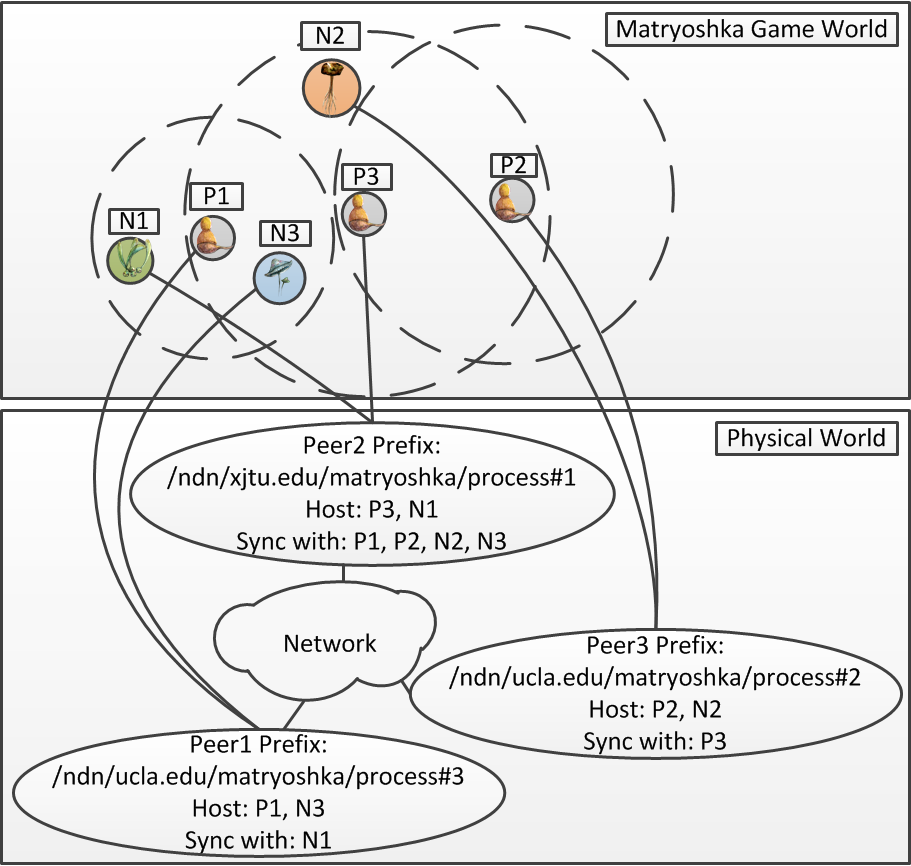
\includegraphics[width=0.75\textwidth]{ProblemDemo.png}
	\caption{游戏应用的局部性要求}
	\label{fig:Locality}
\end{figure}
\par
图\ref{fig:Locality}体现了分布式虚拟环境。P3应该发现P1、P2和N2、N3。P1、P2分别由Peer1和Peer3主持。对于这样的情况,Peer2如何通过向网络进行询问,了解到上述四个点的信息或名称,而不包括N1的信息,即为局部性要求的体现。
\subsubsection{实时性(Realtime-ness)}
\par
当对象移动或是做出动作时, 每个对其感兴趣的节点,即包含该对象在自己的感知范围内的节点,应当尽快的获得关于移动或是动作的更新。特别是当一个对象从一个节点的感知范围外移动到感知范围内,或是从感知范围内移动到感知范围外,即加入和离开事件发生时,节点应该尽可能早的获悉事件的发生。
\subsubsection{大规模可拓展性(Scalability)}
\par
由于本项目旨在解决大规模网络游戏的联机问题,只要不是用户主观需求,所有节点应当尽可能的处于同一个虚拟世界中,因此大规模可拓展性是设计方案中需要考虑的。这一点体现在NDN网络中即为尽可能多的利用节点的数据缓存中的信息,通过全局共享的命名空间,实现在满足实时性的同时存在最大规模的数据共享。
\subsubsection{健壮性(Robustness)}
\par
在实际网络环境中,分块、丢包、乱序、掉线等异常时有发生。由于当前的客户端函数库是基于TCP协议的,协议本身对传输质量有保证,这些情况的发生并不应该起到很大影响。但是,考虑到TCP协议的头部较大,影响传输效率,实际实现会采用UDP协议。同时,理论NDN架构并不基于TCP,理论NDN网络层也是无状态的,不提供针对丢包、乱序的处理。综上,更高层的协议,即游戏应用通讯的应用层协议,应当为这些异常情况负责。游戏应用应当在出现丢包、乱序时尽可能的自行做出处理,并在侦测到对象掉线后予以删除。
\section{系统框架}
\setcounter{subsubsection}{0}
\par
需求分析中根据系统的逻辑功能,将系统划分为如下几个模块。
\begin{figure}[h!]
	\centering
	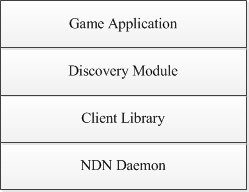
\includegraphics[width=0.40\textwidth]{ApplicationStructure.png}
	\caption{系统框架层次图}
	\label{fig:AbstractStructure}
\end{figure}
\par
\subsubsection{NDND(NDN Daemon)}
\par
运行在各个节点负责NDN路由等节点逻辑的NDN进程。当前最新的NDND是NFD\footnote{NFD的介绍和源码,https://github.com/named-data/NFD},本应用支持的时ndnd-tlv\footnote{ndnd-tlv的介绍和源码,https://github.com/named-data/ndnd-tlv},本应用早期的版本基于的是ccnd\footnote{ccnd的介绍和源码,https://github.com/ProjectCCNx/ccnx}。
\subsubsection{开发者函数库}
\par
如前面所介绍,开发者函数库为NDN应用封装了NDN提供的功能。
\subsubsection{同步模块}
\par
同步模块是在开发者函数库之上,独立于游戏应用之外的函数库。同步模块实现分布式虚拟环境的发现、更新的功能。将同步模块分离的意义的在于别的类似功能的应用可以直接使用该模块,而不必担心和游戏应用的耦合。
\subsubsection{游戏应用}
\par
游戏应用负责渲染、插值、预估等功能。其调用同步模块提供的功能,决定渲染哪些对象。
\section{本章小结}
本章描述了系统的四大需求,局部性、实时性、可拓展性和健壮性。在此之后,本章给出了系统的大致框架,本文需要实现的主要部分在于框架的上三层,需要设计的部分在于框架的上两层。下面的本文的重点将在同步模块的设计、评估和改良上。

